\newpage 

\myWideProblem{
    Read the last two questions on the last page very closely.
    I used the word ``suggests''. 
    What am I trying to emphasize when I use that word?
}
{1in}

\myWideProblem{
    Answer these questions about \nameref{sec:prob-3}.
    \begin{itemize}[nosep]
        \item What date (month \& year) does $x=0$ correspond to? \gap{June 2023}
        \item What is the value of your cubic regression equation when $x=0$? \gap{$y=-12.63$}
        \item Does a model of hospitalizations ``make sense'' the value of $y$ is negative? Why or why not.
    \end{itemize}
}
{1in}

\myWideProblem{
    What difference do you think I mean when I say ``estimate'' and ``predict''?
}
{1in}

% \myWideProblem{
%     Can we use a regression equation to reliably predict the CDC hospitalization data 
%     \myEmph{far} into the future? Why or why not?
% }
% {1in}

\myWideProblemWithContent{
    Here is a screenshot of the CDC hospitalization data for a larger span of time.
    \begin{center}
        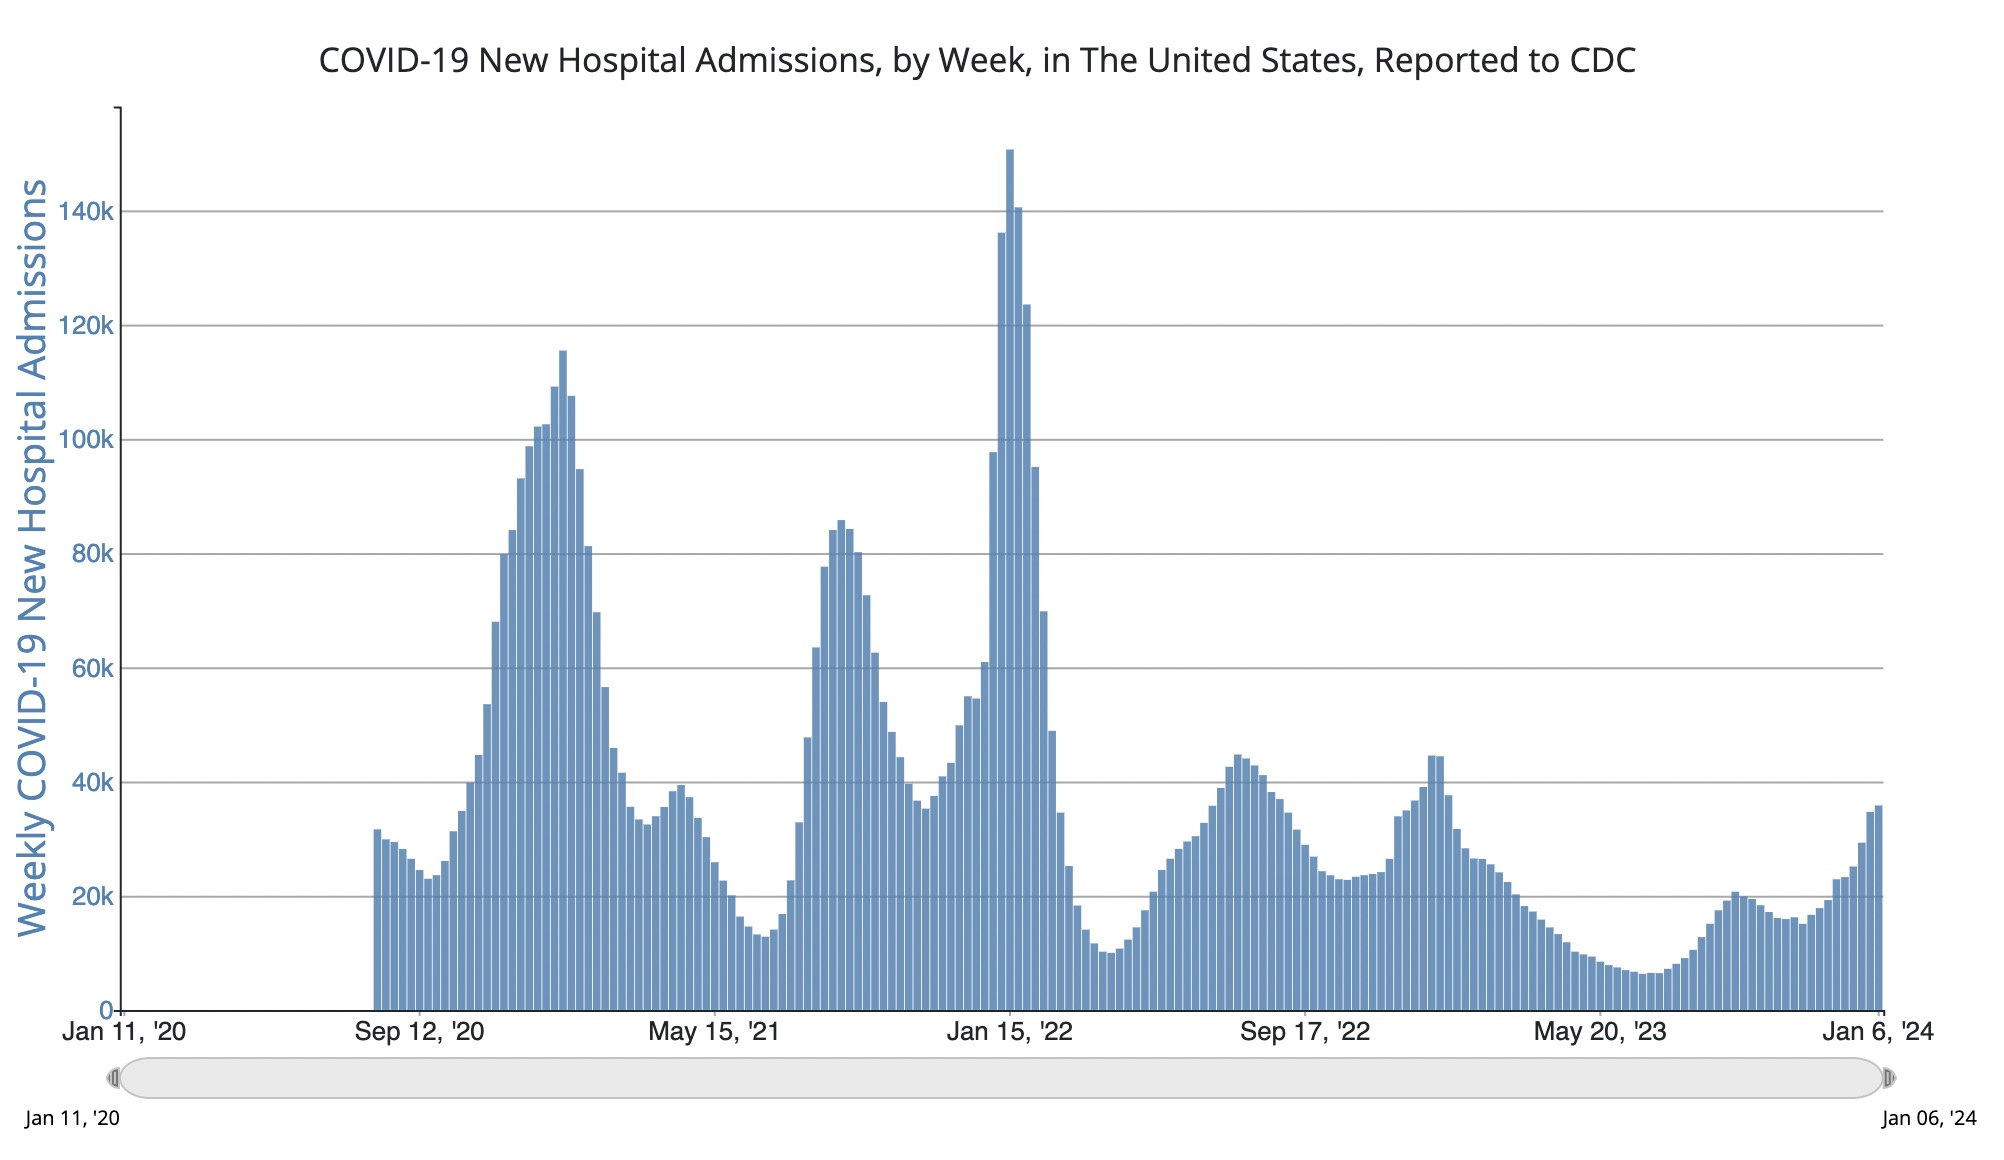
\includegraphics[width=4in,]{hospitalizations-graph.jpg}
    \end{center}
    Does this look linear or quadratic or cubic? Explain your reasoning.
    \vspace{0.65in}
}